\begin{titlepage}
\begin{center}
    \vspace*{1.0cm}

    {\fontsize{16}{22}\selectfont\bfseries\color{rbruNavy} ฟิสิกส์เกษตรดิจิทัลและการเรียนรู้เชิงลึก}\par
    \vspace{0.35cm}
    {\fontsize{15}{21}\selectfont\bfseries\color{rbruBlue} การพัฒนาแอปพลิเคชันสมาร์ตโฟนวิเคราะห์ค่ากรด-ด่างของดิน}\par
    \vspace{0.25cm}
    {\fontsize{13.5}{19}\selectfont\bfseries\color{rbruTeal} ชดเชยค่าความคลาดเคลื่อนอุณหภูมิและความชื้นด้วยโครงข่ายประสาทเทียมอิงฟิสิกส์}\par
    \vspace{0.3cm}
    {\fontsize{9.5}{13.5}\selectfont\itshape\color{rbruSlate} (Digital Agriphysics and Deep Learning: Smartphone Application Development for Soil pH Analysis\\with Temperature and Moisture Compensation via Physics-Informed Neural Networks)}\par

    \vspace{0.7cm}
    {\color{rbruGold}\rule{0.65\textwidth}{2.0pt}}\par
    \vspace{0.7cm}

    \begin{figure}[H]
        \centering
        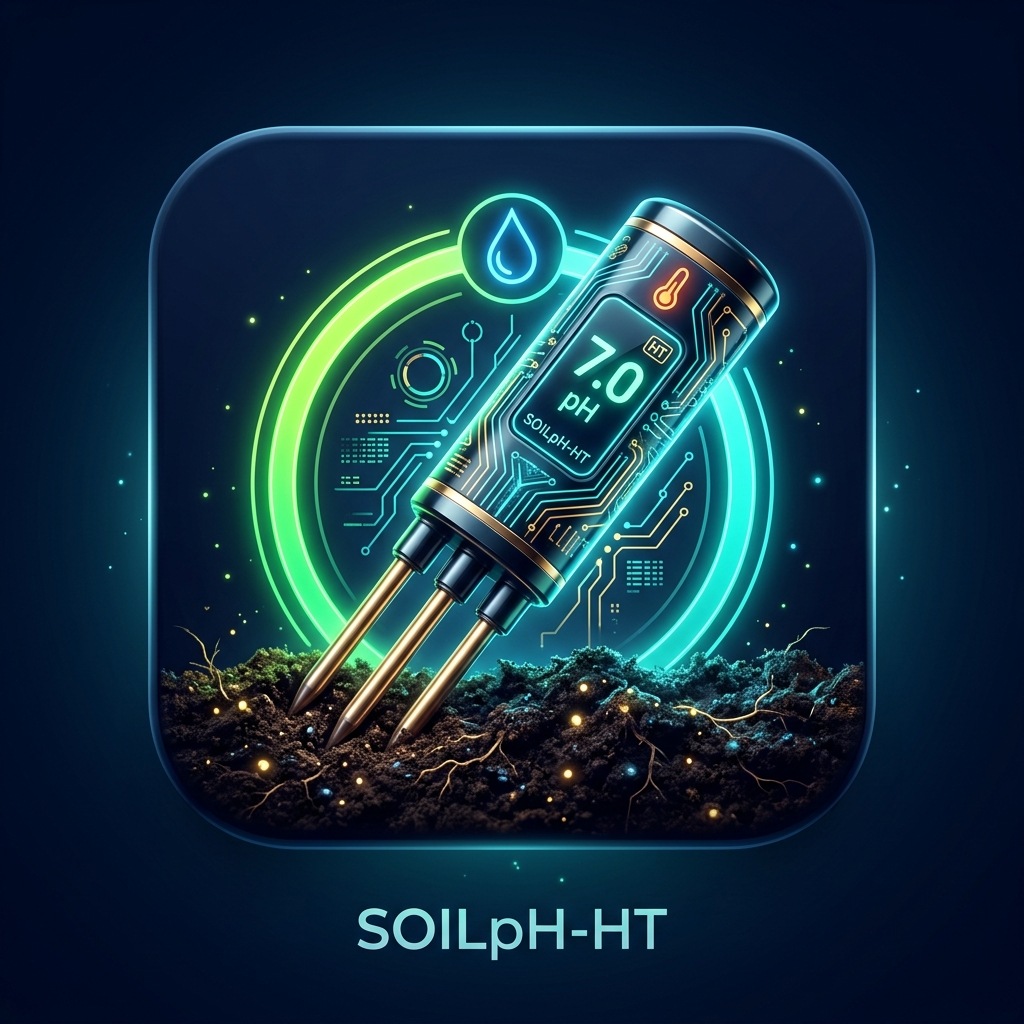
\includegraphics[width=0.35\textwidth]{figures/app_icon.jpg}
    \end{figure}

    \vspace{0.5cm}

    {\fontsize{18}{22}\selectfont\bfseries ผู้ช่วยศาสตราจารย์ ดร.ชีวะ ทัศนา}\par
    \vspace{0.3cm}
    {\fontsize{14}{18}\selectfont สาขาวิชาฟิสิกส์ คณะวิทยาศาสตร์และเทคโนโลยี}\par
    \vspace{0.15cm}
    {\fontsize{14}{18}\selectfont มหาวิทยาลัยราชภัฏรำไพพรรณี}\par
    \vspace{0.8cm}

    {\small พุทธศักราช 2569}

\end{center}
\end{titlepage}
